\chapter{Screen-shots}
\label{screenshots}

\begin{figure}[h!]
\centering
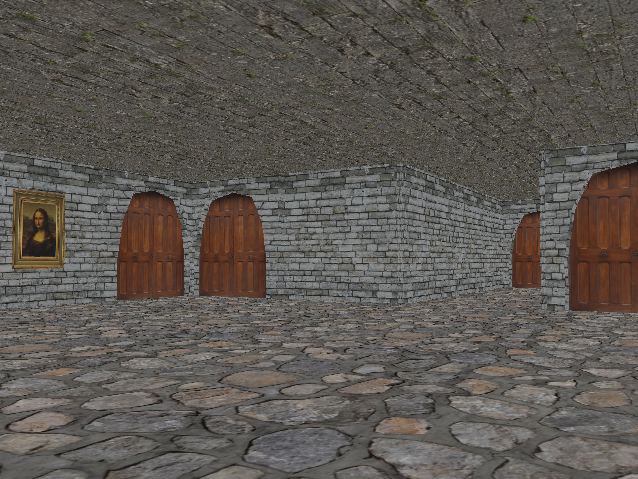
\includegraphics[width=0.49\textwidth]{images/dungeon02.png}
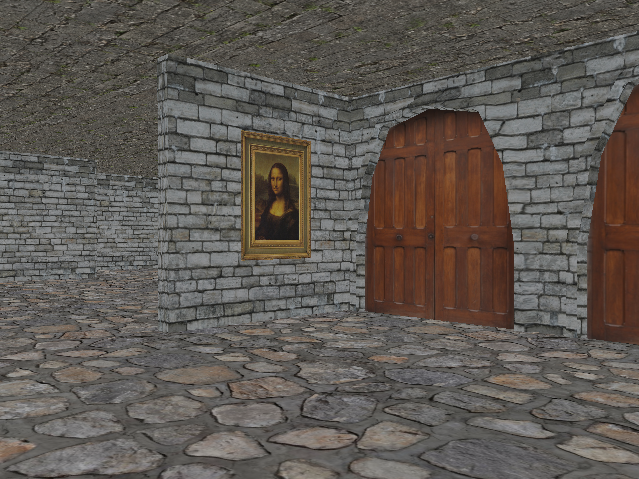
\includegraphics[width=0.49\textwidth]{images/dungeon03.png}
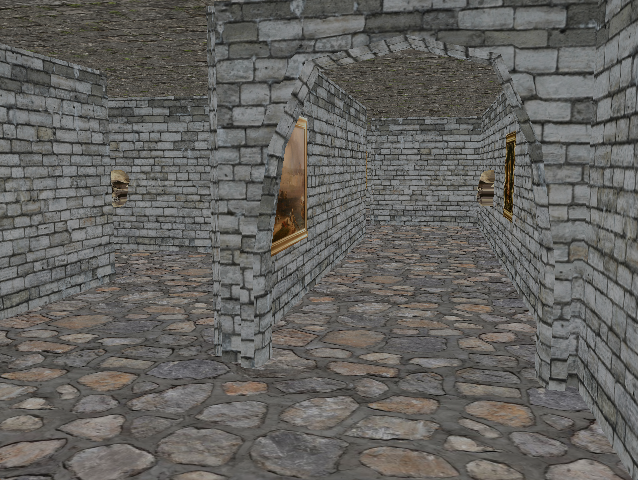
\includegraphics[width=0.49\textwidth]{images/dungeon04.png}
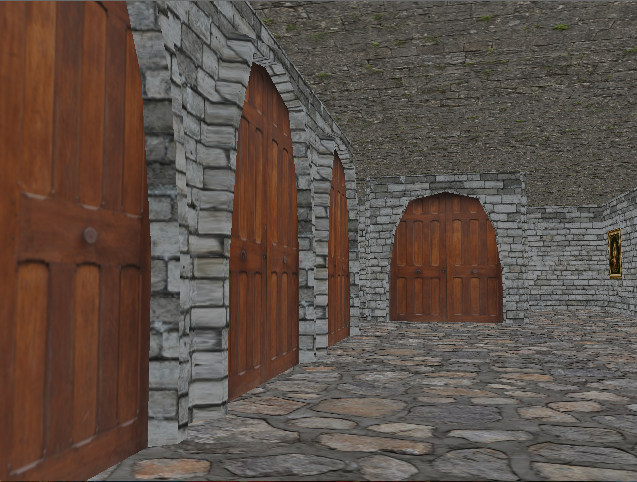
\includegraphics[width=0.49\textwidth]{images/dungeon05.png}
\caption{Screen-shots of the final result.}
\end{figure}

\begin{figure}[h!]
\centering
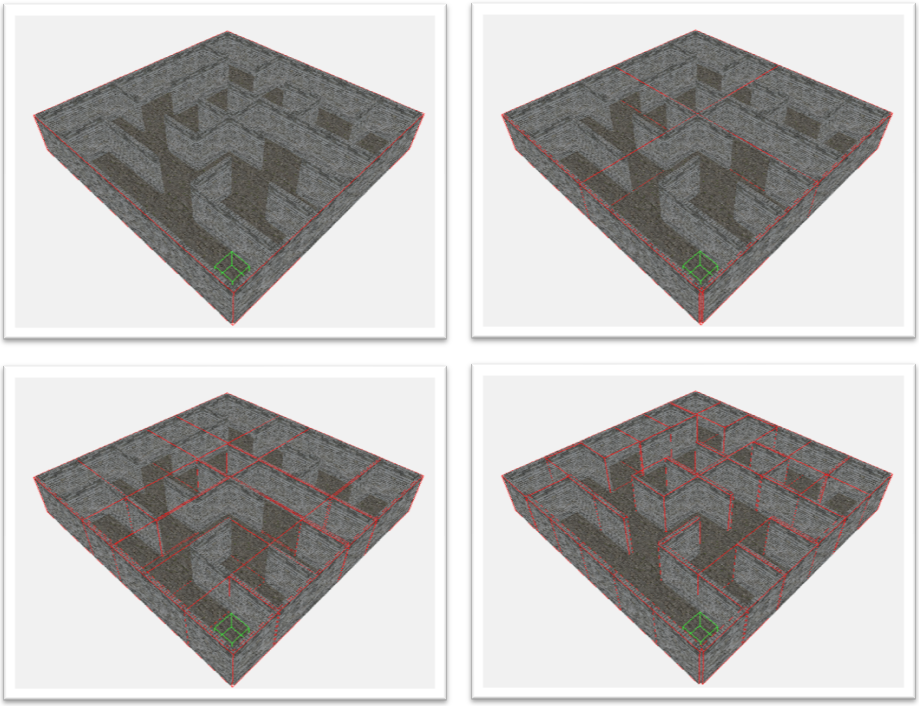
\includegraphics[width=1\textwidth]{images/bvh-depths.png}
\caption{Screen-shots of the BVH at different depths.}
\end{figure}

\begin{figure}[h!]
\centering
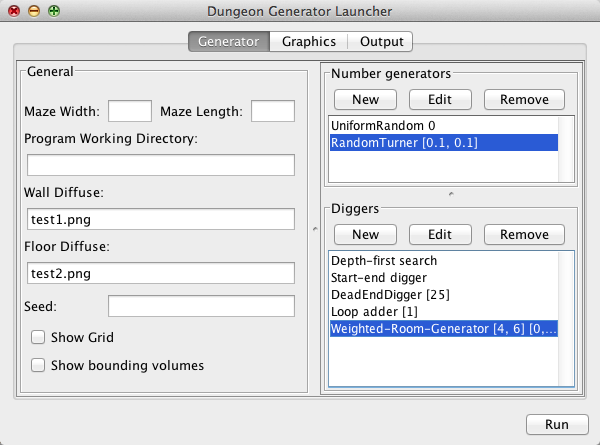
\includegraphics[width=0.49\textwidth]{images/launcher00.png}
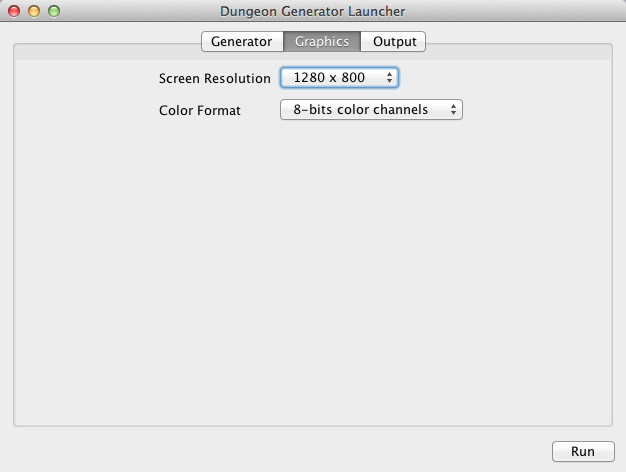
\includegraphics[width=0.49\textwidth]{images/launcher01.png}
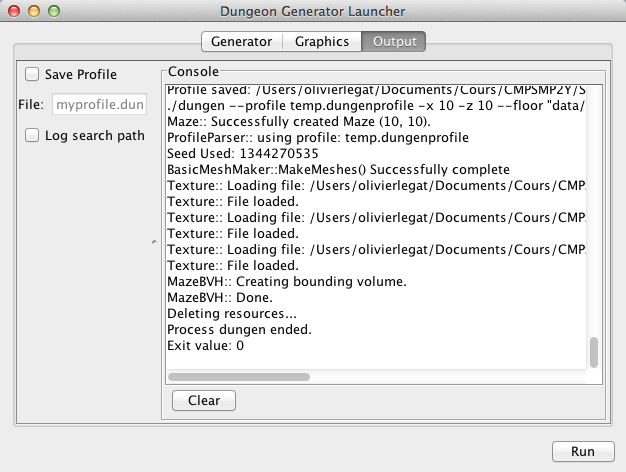
\includegraphics[width=0.49\textwidth]{images/launcher02.png}
\caption{Screen-shots of the launcher.}
\end{figure}








\chapter{Code and Class Diagrams}
\label{codeDiagrams}

\section{Class Diagrams}
\subsection{DunGen}
\begin{figure}[h!]
\centering
 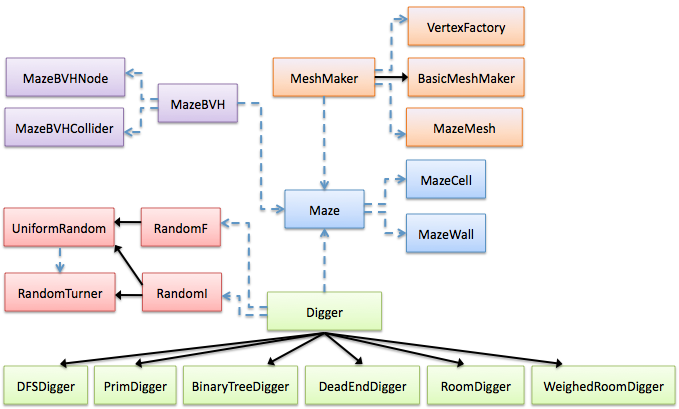
\includegraphics[width=0.80\textwidth]{images/uml_generator0.png}
\caption{Class diagram of the generator structure.}
\end{figure}

\pagebreak
\begin{figure}[h!]
\centering
 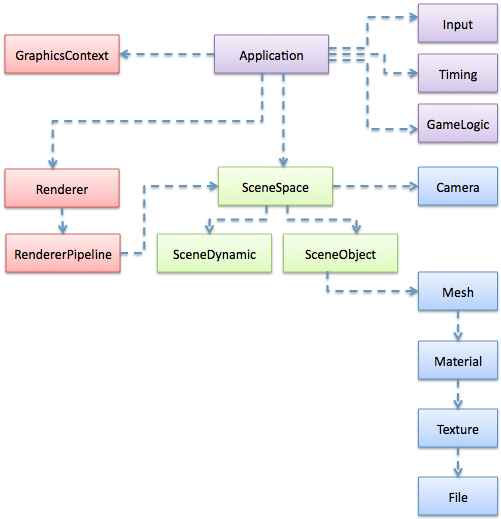
\includegraphics[width=0.65\textwidth]{images/uml_engine0.png}
\caption{Class diagram of the engine structure.}
\end{figure}

\pagebreak
\subsection{Launcher}
\begin{figure}[h!]
\centering
 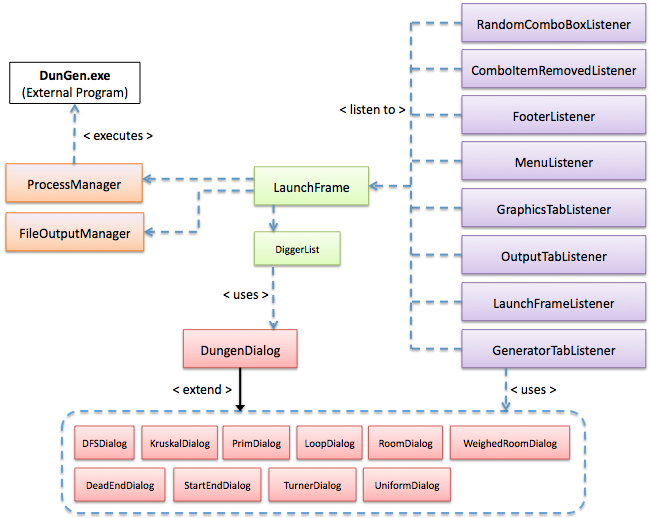
\includegraphics[width=0.78\textwidth]{images/uml_launcher0.png}
\caption{Class diagram of the launcher's structure.}
\end{figure}


\section{Code Listings}
The code listing in this appendix does not cover all the code of project. Only the critical sections that are discussed thoroughly in the dissertation are displayed here.

\subsection {Maze cells and walls}
\lstCpp
\begin{lstlisting}[caption= The \texttt{MazeCell} class]
enum MazeCellType
{
    MAZE_CELL_WALL,
    MAZE_CELL_FLOOR
};

class MazeCell
{
public:
    MazeCell(int x, int z, MazeCellType type);
    ~MazeCell();
    
    bool IsVisited() const {return visited;}
    void SetVisited(const bool b) {visited = b;}
    
    MazeCellType GetCellType() const {return type;}
    void SetCellType(MazeCellType celltype) {type = celltype;}
    
    int X() const {return x;}
    int Z() const {return z;}
    
    Object* GetObject() const {return obj;}
    void SetObject(Object* o) {this->obj = o;}
    
private:
    int x, z;
    MazeCellType type;
    bool visited;
    Object* obj;
};
\end{lstlisting}

\lstCpp
\begin{lstlisting}[caption= The \texttt{MazeWall} class]
enum MazeWallType
{
    MAZE_WALLTYPE_NONE,
    MAZE_WALLTYPE_DEFAULT
};

enum MazeWallPosition
{
    MAZE_WALLPOS_UP,
    MAZE_WALLPOS_DOWN,
    MAZE_WALLPOS_LEFT,
    MAZE_WALLPOS_RIGHT
};

class MazeWall
{
public:
    MazeWall();
    ~MazeWall();
    
    MazeWallType GetType() const { return type; }
    void SetType(MazeWallType t) {type = t;}
    
private:
    MazeWallType type;
};
\end{lstlisting}

\subsection {Maze}
\lstCpp
\begin{lstlisting}[caption= The \texttt{Maze} class]
class Maze
{
public:
    Maze(int width, int length);
    ~Maze();
    
    /**
     * Get a cell.
     * @param A pointer to cell. If [x,z] is out of range, NULL is returned.
     */
    MazeCell* GetCell(const int x, const int z) const;
    MazeWall* GetWall(const MazeCell* cell, MazeWallPosition pos) const;
    MazeWall* GetWall(const int x, const int z, MazeWallPosition pos) const;
    
    MazeWall* GetVWall(const int x, const int z) const {return vwalls[x + z * (width+1)];};
    MazeWall* GetHWall(const int x, const int z) const {return hwalls[x + z * (width)];};
    
    /**
     * Get the cells above and below of the horizontal wall (x, z).
     * @param (x,z) A h-wall's coordinates.
     * @param top [output] Cell above the h-wall (x,z).
     * @param bottom [output] Cell below the h-wall (x,z).
     */
    void GetTopAndBottomCell(const int x, const int z, MazeCell** top, MazeCell** bottom) const;
    
    /**
     * Get the cells on the left and right of the vertical wall (x, z).
     * @param (x,z) A v-wall's coordinates.
     * @param left [output] Cell on the left of the v-wall (x,z).
     * @param right [output] Cell on the right of the v-wall (x,z).
     */
    void GetLeftAndRightCell(const int x, const int z, MazeCell** left, MazeCell** right) const;
    
    /**
     * Break the wall between two adjacent cells (i.e. Set it to WALLTYPE_NONE).
     *
     * @param cell1 Any cell.
     * @param cell2 Any cell.
     */
    void BreakWalls(const MazeCell* cell1, const MazeCell* cell2);
    
    /**
     * Break all the vertical walls within the region of cell1 and cell2 (excluding borders)
     * @param cell1 Any cell.
     * @param cell2 Any cell.
     */
    void BreakVWalls(const MazeCell* cell1, const MazeCell* cell2);
    
    /**
     * Break all the horizontal walls within the region of cell1 and cell2 
     * (excluding borders)
     * @param cell1 Any cell.
     * @param cell2 Any cell.
     */
    void BreakHWalls(const MazeCell* cell1, const MazeCell* cell2);
    
    /**
     * @return true if cell1 and cell2 are adjacent (i.e. x, z indices differ by 1 exactly)
     */
    bool AreAdjacent(const MazeCell* cell1, const MazeCell* cell2) const;
    
    /**
     * @param cell Which cell to wall off completely. This cell is set to MAZE_CELL_WALL.
     */
    void WallOff(MazeCell* cell);
    
    /**
     * @param cell Any cell.
     * @return The number of walls this cell is touching.
     */
    int GetWallCount(const MazeCell* cell) const;
    
    /**
     * @return True if cell is considered a dead-end (i.e. wall count = 3).
     */
    bool IsDeadEnd(const MazeCell* cell) const {return GetWallCount(cell) == 3;}
    
    /**
     * @return True if their are no walls in between cell1 to cell2.
     */
    bool IsRoom(const MazeCell* cell1, const MazeCell* cell2);
    
    int Width() const {return width;}
    int Length() const {return length;}
    
    int VWallWidth() const {return width + 1;}
    int VWallLength() const {return length;}
    
    int HWallWidth() const {return width;}
    int HWallLength() const {return length + 1;}
    
    /**
     * @param cell Parent cell.
     * @param children [output] An array of atleast an initial size 4. Points to adjacent
     *        unvisited cells. Use NULL if you just want the count.
     * @return number of visited children.
     */
    int GetUnvisitedCells(const MazeCell* cell, MazeCell** children) const;
    
    /**
     * @param cell Parent cell.
     * @param children [output] An array of atleast an initial size 4. Points to adjacent
     *        cells. Use NULL if you just want the count.
     * @return number of adjacent cell.
     */
    int GetAdjacentCells(const MazeCell* cell, MazeCell** children) const;
    
    /**
     * Print maze to file:
     */
    void Print(FILE* output) const;
    
    /**
     * Print maze to stdout:
     */
    void Print() const;
    
private:
    int width;
    int length;
    
    Array<MazeCell*> cells;
    Array<MazeWall*> vwalls;
    Array<MazeWall*> hwalls;
    
    void printHWall(FILE* output, int x, int z) const;
    void printVWall(FILE* output, int x, int z) const;
    void printCell (FILE* output, int x, int z) const;
};

\end{lstlisting}

\subsection{Mesh generation}
All the classes used to generate the 3D mesh are in {\em Generator/MazeMesh/} where the class \texttt{MazeMesh} can be found. This class is a simplified version of the \texttt{Mesh} class in the engine and it used to hold data of the created meshes. The reason for using the different class is to keep the generator engine-independent. The \texttt{Mesh} class will have functionality that concerns rendering modes and the material used, whereas the \texttt{MazeMesh} is only concerned about the vertices of the mesh.

The class used to implement the mesh generation is the \texttt{BasicMeshMaker} that implements the \texttt{MeshMaker} interface, both found in {\em Generator/MazeMesh/MeshMaker/}. This mesh generator uses the \texttt{VertexFactory} class to construct a series of boxes for the walls of the maze, it also creates a plane for the floor. The generator builds the vertex position array, the index array and texture coordinate array of the mesh and sub-meshes.
\lstCpp
\begin{lstlisting}[caption= The \texttt{VertexFactory} class]
void VertexFactory::ToArray(List<float> &l, Array<float> &a) {
    a = Array<float>(l.size());
    
    int i = 0;
    List<float>::iterator it;
    for (it = l.begin(); it != l.end(); it++)
        a[i++] = * it;
}
void VertexFactory::ToArray(List<int> &l, Array<int> &a) {
    a = Array<int>(l.size());
    
    int i = 0;
    List<int>::iterator it;
    for (it = l.begin(); it != l.end(); it++)
        a[i++] = * it;
}

void VertexFactory::MergeVertices(List<float> &verts1, List<int> &inds1,
                                  const Array<float> &verts2, const Array<int> &inds2)
{
    int i, ioff = (int) verts1.size();
    
    for (i = 0; i < verts2.size(); i++) verts1.push_back(verts2[i]);
    for (i = 0; i < inds2.size(); i++) inds1.push_back(inds2[i] + ioff);
}

void VertexFactory::MergeVertices(const Array<float> &verts1, const Array<int> &inds1,
                          const Array<float> &verts2, const Array<int> &inds2,
                          Array<float> &out_verts, Array<int> &out_inds) 
{
    int i, voff = (int) verts1.size(), ioff = (int) verts2.size();
    
    out_verts = Array<float>(verts1.size() + verts2.size());
    out_inds  = Array<int>( inds1.size() +  inds2.size());
    
    for (i = 0; i < verts1.size(); i++) out_verts[i] = verts1[i];
    for (i = 0; i < inds2.size();  i++) out_inds[i]  = inds1[i];
    
    for (i = 0; i < verts2.size(); i++) out_verts[i + voff] = verts2[i];
    for (i = 0; i < inds2.size();  i++) out_inds[i + ioff] = inds2[i] + voff;
}


void VertexFactory::CreatePlane(Array<float> &vertices, Array<int> &indices, 
                                Vector3 o, Quaternion r, float w, float l, int dw, int dl, int mode)
{
    int ix, iz;
    int nx = dw + 1; // number of verts in the x-axis.
    int nz = dl + 1; // number of verts in the z-axis.
    
    // TODO: optimize... init vertices, indices once (no push_back)
    
    float x = o.x - (w / 2.0f); // init x-coord of first vertex.
    float y = o.y;
    float z;
    
    // Create vertices.
    for (ix = 0; ix < nx; ix++) // For each vertex.
    {
        // Reset the z-coord. for this row.
        z = o.z - (l / 2.0f);
        
        for (iz = 0; iz < nz; iz++) 
        {
            // Rotate the vertex:
            Vector3 v = Vector3(x, y, z);
            v = v - o; // Bring to 0,0,0
            v = v * r; // rotate
            v = v + o; // shift back to ox,oy,oz
            
            // Add the vertex:
            vertices.push_back(v.x);
            vertices.push_back(v.y);
            vertices.push_back(v.z);
            
            // Shift the z-coord. for the next vertex.
            z += l / dl;
        }
        
        // Shift the x-coord. for the next row of vertices.
        x += w / dw;
    }
    
    // Create indices:
    for (ix = 0; ix < dw; ix++) // For each square.
        for (iz = 0; iz < dl; iz++)
        {
            /*               .---.
             *               |   |
             * (ix, iz) --> (.)--.
             */
            
            // Get indices
            int bl = iz + (ix * nz);       // bottom-left index.
            int br = iz + ((ix+1) * nz);   // bottom-right index.
            int tl = iz+1 + (ix * nz);     // top-left index.
            int tr = iz+1 + ((ix+1) * nz); // top-right index.
            
            switch (mode) 
            {
                case GL_QUADS:
                    // Add a quad:
                    indices.push_back(bl * 3);
                    indices.push_back(tl * 3);
                    indices.push_back(tr * 3);
                    indices.push_back(br * 3);
                    break;
            
                case GL_TRIANGLES:
                default:
                    // Add 2 triangles:
                    indices.push_back(tr * 3);
                    indices.push_back(br * 3);
                    indices.push_back(bl * 3);
                    
                    indices.push_back(tr * 3);
                    indices.push_back(bl * 3);
                    indices.push_back(tl * 3);
                    break;
            }
        }
}

void VertexFactory::CreateCuboid(Array<float> &vertices, Array<int> &indices,
                                 Vector3 o, Quaternion r, Vector3 v, int dw, int dh, int dl, int mode)
{
    List<float> lvertices = List<float>();
    List<int> lindices = List<int>();
    Array<float> planeVerts = Array<float>();
    Array<int> planeInds = Array<int>();
    Vector3 center; // center of the plane
    Quaternion orient; // orientation of the plane
    
    // Make front face:
    center = o + Vector3(0, 0, v.z / 2.0f);
    orient = Quaternion(Vector3( - PI / 2, 0, 0));
    CreatePlane(planeVerts, planeInds, center, orient, v.x, v.y, dw, dh, mode);
    MergeVertices(lvertices, lindices, planeVerts, planeInds);
    planeVerts.clear();
    planeInds.clear();
    
    // Make back face:
    center = o - Vector3(0, 0, v.z / 2.0f);
    orient = Quaternion(Vector3( PI / 2, 0, 0));
    CreatePlane(planeVerts, planeInds, center, orient, v.x, v.y, dw, dh, mode);
    MergeVertices(lvertices, lindices, planeVerts, planeInds);
    planeVerts.clear();
    planeInds.clear();
    
    // Make left face:
    center = o + Vector3(v.x / 2.0f, 0, 0);
    orient = Quaternion(Vector3( 0, 0, PI / 2));
    CreatePlane(planeVerts, planeInds, center, orient, v.y, v.z, dh, dl, mode);
    MergeVertices(lvertices, lindices, planeVerts, planeInds);
    planeVerts.clear();
    planeInds.clear();
    
    // Make right face:
    center = o - Vector3(v.x / 2.0f, 0, 0);
    orient = Quaternion(Vector3( 0, 0, -PI / 2));
    CreatePlane(planeVerts, planeInds, center, orient, v.y, v.z, dh, dl, mode);
    MergeVertices(lvertices, lindices, planeVerts, planeInds);
    planeVerts.clear();
    planeInds.clear();
    
    // Make top face:
    center = o + Vector3(0, v.y / 2.0f, 0);
    orient = Quaternion(Vector3( 0, 0, 0) );
    CreatePlane(planeVerts, planeInds, center, orient, v.x, v.z, dw, dl, mode);
    MergeVertices(lvertices, lindices, planeVerts, planeInds);
    planeVerts.clear();
    planeInds.clear();
    
    // Make bottom face:
    center = o - Vector3(0, v.y / 2.0f, 0);
    orient = Quaternion(Vector3( PI , 0, 0) );
    CreatePlane(planeVerts, planeInds, center, orient, v.x, v.z, dw, dl, mode);
    MergeVertices(lvertices, lindices, planeVerts, planeInds);
    planeVerts.clear();
    planeInds.clear();
    
    // Convert lists into arrays:
    VertexFactory::ToArray(lvertices, vertices);
    VertexFactory::ToArray(lindices, indices);
    
    // Rotate each vertex around the origin o:
    int n = (int) vertices.size();
    for (int i = 0; i < n; i = i + 3)
    {
        Vector3 v = Vector3(vertices[i], vertices[i+1], vertices[i+2]);
        v = v - o;
        v = v * r;
        v = v + o;
        vertices[i]   = v.x;
        vertices[i+1] = v.y;
        vertices[i+2] = v.z;
    }
}
\end{lstlisting}

\lstCpp
\begin{lstlisting}[caption= The \texttt{BasicMeshMaker} class]
void BasicMeshMaker::makeWallVertices(List<float> &verts, List<int> &inds, List<float> &texcoords)
{
    unsigned int x, z, n, m;
    MazeWall* wall;
    
    // Init wall data arrays:
    Array<float> wallVerts = Array<float>();
    Array<int> wallInds = Array<int>();
    
    // For each horizontal wall:
    n = maze->HWallWidth();
    m = maze->HWallLength();
    for (x = 0; x < n; x++)
        for ( z = 0; z < m; z++)
        {
            wall = maze->GetHWall(x, z);
            if (wall->GetType() == MAZE_WALLTYPE_NONE) continue; // No wall. Ditch.
            
            Vector3 o; // center of the wall (pivot point, origin).
            o.x = position.x + (width * x) + width / 2;
            o.y = position.y + height / 2;
            o.z = position.z + (length * z);
            Quaternion r = Quaternion(Vector3(0));
            
            VertexFactory::CreateCuboid(wallVerts, wallInds, o, r, Vector3(width, height, wallThickness),
                                        1, 1, 1, primitiveType);
            VertexFactory::MergeVertices(verts, inds, wallVerts, wallInds);
            
            {
                // Front face
                texcoords.push_back(0.0f); texcoords.push_back(0.0f);
                texcoords.push_back(0.0f); texcoords.push_back(1.0f);
                texcoords.push_back(1.0f); texcoords.push_back(0.0f);
                texcoords.push_back(1.0f); texcoords.push_back(1.0f);
                
                // Back face (mirrored vertically)
                texcoords.push_back(1.0f); texcoords.push_back(1.0f);
                texcoords.push_back(1.0f); texcoords.push_back(0.0f);
                texcoords.push_back(0.0f); texcoords.push_back(1.0f);
                texcoords.push_back(0.0f); texcoords.push_back(0.0f);
                
                // Left face (flipped 90°)
                texcoords.push_back(0.0f); texcoords.push_back(0.0f);
                texcoords.push_back(1.0f); texcoords.push_back(0.0f);
                texcoords.push_back(0.0f); texcoords.push_back(1.0f);
                texcoords.push_back(1.0f); texcoords.push_back(1.0f);
                
                // Right face (flipped 270°)
                texcoords.push_back(1.0f); texcoords.push_back(1.0f);
                texcoords.push_back(0.0f); texcoords.push_back(1.0f);
                texcoords.push_back(1.0f); texcoords.push_back(0.0f);
                texcoords.push_back(0.0f); texcoords.push_back(0.0f);
                
                // Top face (flipped 90°)
                texcoords.push_back(0.0f); texcoords.push_back(0.0f);
                texcoords.push_back(1.0f); texcoords.push_back(0.0f);
                texcoords.push_back(0.0f); texcoords.push_back(1.0f);
                texcoords.push_back(1.0f); texcoords.push_back(1.0f);
                
                // Bottom face
                texcoords.push_back(0.0f); texcoords.push_back(0.0f);
                texcoords.push_back(0.0f); texcoords.push_back(1.0f);
                texcoords.push_back(1.0f); texcoords.push_back(0.0f);
                texcoords.push_back(1.0f); texcoords.push_back(1.0f);
            }
            
            wallVerts.clear();
            wallInds.clear();
        }
    
    
    // For each horizontal wall:
    n = maze->VWallWidth();
    m = maze->VWallLength();
    for (x = 0; x < n; x++)
        for ( z = 0; z < m; z++)
        {
            wall = maze->GetVWall(x, z);
            if (wall->GetType() == MAZE_WALLTYPE_NONE) continue; // No wall. Ditch.
            
            Vector3 o; // center of the wall (pivot point, origin).
            o.x = position.x + (width * x);
            o.y = position.y + height / 2;
            o.z = position.z + (length * z) + length / 2;
            Quaternion r = Quaternion(Vector3(0));
            
            VertexFactory::CreateCuboid(wallVerts, wallInds, o, r, Vector3(wallThickness, height, length),
                                        1, 1, 1, primitiveType);
            VertexFactory::MergeVertices(verts, inds, wallVerts, wallInds);
            
            {
                // Front face
                texcoords.push_back(0.0f); texcoords.push_back(0.0f);
                texcoords.push_back(0.0f); texcoords.push_back(1.0f);
                texcoords.push_back(1.0f); texcoords.push_back(0.0f);
                texcoords.push_back(1.0f); texcoords.push_back(1.0f);
                
                // Back face (mirrored vertically)
                texcoords.push_back(1.0f); texcoords.push_back(1.0f);
                texcoords.push_back(1.0f); texcoords.push_back(0.0f);
                texcoords.push_back(0.0f); texcoords.push_back(1.0f);
                texcoords.push_back(0.0f); texcoords.push_back(0.0f);
                
                // Left face (flipped 90°)
                texcoords.push_back(0.0f); texcoords.push_back(0.0f);
                texcoords.push_back(1.0f); texcoords.push_back(0.0f);
                texcoords.push_back(0.0f); texcoords.push_back(1.0f);
                texcoords.push_back(1.0f); texcoords.push_back(1.0f);
                
                // Right face (flipped 270°)
                texcoords.push_back(1.0f); texcoords.push_back(1.0f);
                texcoords.push_back(0.0f); texcoords.push_back(1.0f);
                texcoords.push_back(1.0f); texcoords.push_back(0.0f);
                texcoords.push_back(0.0f); texcoords.push_back(0.0f);
                
                // Top face
                texcoords.push_back(0.0f); texcoords.push_back(0.0f);
                texcoords.push_back(0.0f); texcoords.push_back(1.0f);
                texcoords.push_back(1.0f); texcoords.push_back(0.0f);
                texcoords.push_back(1.0f); texcoords.push_back(1.0f);
                
                // Bottom face
                texcoords.push_back(0.0f); texcoords.push_back(0.0f);
                texcoords.push_back(0.0f); texcoords.push_back(1.0f);
                texcoords.push_back(1.0f); texcoords.push_back(0.0f);
                texcoords.push_back(1.0f); texcoords.push_back(1.0f);
            }
            
            wallVerts.clear();
            wallInds.clear();
        }
}

void BasicMeshMaker::makeFloorVertices(Array<float> &verts, Array<int> &inds, Array<float> &texcoords)
{
    // Calculate width / length of the mesh.
    float totalWidth = width * maze->Width();
    float totalLength = length * maze->Length();
    
    Vector3 o = position + Vector3(totalWidth / 2.0f, 0, totalLength / 2.0f);
    
    VertexFactory::CreatePlane(verts, inds, o, Quaternion(Vector3(0)),
                               totalWidth, totalLength, 1, 1, primitiveType);
    
    texcoords.push_back(0.0f); texcoords.push_back(0.0f);
    texcoords.push_back(0.0f); texcoords.push_back(totalLength);
    texcoords.push_back(totalWidth); texcoords.push_back(0.0f);
    texcoords.push_back(totalWidth); texcoords.push_back(totalLength);
}

void BasicMeshMaker::makeCeilingVertices(Array<float> &verts, Array<int> &inds, Array<float> &texcoords)
{
    // Calculate width / length of the mesh.
    float totalWidth = width * maze->Width();
    float totalLength = length * maze->Length();
    
    Vector3 o = position + Vector3(totalWidth / 2.0f, 1, totalLength / 2.0f);
    
    VertexFactory::CreatePlane(verts, inds, o, Quaternion(Vector3(PI, 0, 0)),
                               totalWidth, totalLength, 1, 1, primitiveType);
    
    texcoords.push_back(0.0f); texcoords.push_back(0.0f);
    texcoords.push_back(0.0f); texcoords.push_back(totalLength);
    texcoords.push_back(totalWidth); texcoords.push_back(0.0f);
    texcoords.push_back(totalWidth); texcoords.push_back(totalLength);
}
\end{lstlisting}

\subsection{Number Generator}
\lstCpp
\begin{lstlisting}
#define MAZE_LCG_A 16807      // 7^5
#define MAZE_LCG_M 2147483647 // 2^31 - 1
#define MAZE_LCG_C 0          // 0

int UniformRandom::nextInt()
{
    x = (x * MAZE_LCG_A + MAZE_LCG_C) % MAZE_LCG_M;
    return (int) ( x & 0x00FF );
}

int UniformRandom::nextInt(int max)
{
    return nextInt(0, max);
}

int UniformRandom::nextInt(int min, int max)
{
    assert(max > 0);
    assert(min >= 0);
    int l = max - min; if(l < 0) l *= -1;
    return ((int) nextInt() % l) + min;
}

float UniformRandom::nextFloat()
{
    return nextFloat(0.0f, 1.0f);
}

float UniformRandom::nextFloat(float max)
{
    assert(max >= 0.0f);
    return nextFloat(0.0f, max);
}

float UniformRandom::nextFloat(float min, float max)
{
    assert(min <= max);
    /* calculate the random number & return it */
	return ((float)rand() / (static_cast<float>(RAND_MAX) + 1.0f))
	* (max - min) + min;
}
\end{lstlisting}

\subsection{Collider}
\lstCpp
\begin{lstlisting}[caption=The \texttt{MazeCollider} and \texttt{MazeColliderAABB} classes]
class MazeCollider
{
protected:
    MazeCollider();
    
public:
    ~MazeCollider();
    
    virtual float GetMinX()const =0;
    virtual float GetMinY()const =0;
    virtual float GetMinZ()const =0;
    virtual float GetMaxX()const =0;
    virtual float GetMaxY()const =0;
    virtual float GetMaxZ()const =0;
    
    /**
     * @param maxX [output] set to GetMaxX().
     * @param maxY [output] set to GetMaxY().
     * @param maxZ [output] set to GetMaxZ().
     * @param minX [output] set to GetMinX().
     * @param minY [output] set to GetMinY().
     * @param minZ [output] set to GetMinZ().
     */
    void GetAllMinMax(float* minX, float* minY, float* minZ,
                      float* maxX, float* maxY, float* maxZ) const;
};

class MazeColliderAABB : public MazeCollider
{
public:
    MazeColliderAABB();
    ~MazeColliderAABB();
    
    void    GetVolume(float* x, float* y, float* z);
    Vector3 GetVolume() const { return vol; }
    float GetWidth()  const { return vol.x; }
    float GetLength() const { return vol.z; }
    float GetHeight() const { return vol.y; }
    
    void    GetTranslation(float* x, float* y, float* z);
    Vector3 GetTranslation() const { return trans; }
    float GetX() const { return trans.x; }
    float GetY() const { return trans.y; }
    float GetZ() const { return trans.z; }
    
    void SetVolume(Vector3 v) { this->vol = v; }
    void SetWidth (float x) { this->vol.x = x; }
    void SetLength(float z) { this->vol.z = z; }
    void SetHeight(float y) { this->vol.y = y; }
    
    void SetTranslation(Vector3 t) { this->trans = t; }
    void SetX(float x) { this->trans.x = x; }
    void SetY(float y) { this->trans.y = y; }
    void SetZ(float z) { this->trans.z = z; }
    
    virtual float GetMinX()const {return trans.x - vol.x / 2.0f;}
    virtual float GetMinY()const {return trans.y - vol.y / 2.0f;}
    virtual float GetMinZ()const {return trans.z - vol.z / 2.0f;}
    virtual float GetMaxX()const {return trans.x + vol.x / 2.0f;}
    virtual float GetMaxY()const {return trans.y + vol.y / 2.0f;}
    virtual float GetMaxZ()const {return trans.z + vol.z / 2.0f;}
    
    Vector3 GetMinCorner() const;
    Vector3 GetMaxCorner() const;
    
private:
    Vector3 vol;
    Vector3 trans;
};
\end{lstlisting}

\lstCpp
\begin{lstlisting}[caption=The \texttt{MazeBVHNode} class]
class MazeBVHNode : public Object
{
    friend class MazeBVH;
    
protected:
    MazeBVHNode(MazeBVHNode** children, float childrenCount);
    MazeBVHNode(MazeCollider* collider);
    MazeBVHNode();
    
    /**
     * Delete this node and its collider. Recursively calls ~MazeBVNode()
     * on all its children. Also set parent to NULL.
     */
    ~MazeBVHNode();
    
public:
    int GetChildrenCount() const { return (int) children.size(); }
    MazeBVHNode* GetChild(int index) const { return children[index]; }
    MazeBVHNode* GetParent() const { return parent; }
    MazeCollider* GetCollider() const { return collider; }
    
    bool IsLeaf() const { return GetChildrenCount() == 0; }
    bool IsRoot() const { return parent == NULL; }
    int  GetHeight() const { return height; }
    
private:
    int height;
    MazeCollider* collider;
    MazeBVHNode* parent;
    Array<MazeBVHNode*> children;
};
\end{lstlisting}

\lstCpp
\begin{lstlisting}[caption=The \texttt{MazeBVH} class]
#include "MazeBVH.h"

MazeBVH::MazeBVH() 
{
    this->root = NULL;
}
MazeBVH::~MazeBVH() {}

MazeBVH* MazeBVH::CreateBoundingVolumeHierarchy(BasicMeshMaker* maker)
{
    const Maze* maze = maker->GetMaze();
    MazeCell* c1 = maze->GetCell(0, 0);
    MazeCell* c2 = maze->GetCell(maze->Width()-1, maze->Width()-1);
    
    MazeBVH* bvh = new MazeBVH();
    bvh->root = CreateBVHNode(maker, c1, c2);
    return bvh;
}

MazeBVHNode* MazeBVH::CreateBVHNode(BasicMeshMaker* maker, MazeCell* from, MazeCell* to)
{
    const Maze* maze = maker->GetMaze();
    MazeBVHNode* leaves[4];
    leaves[0] = leaves[1] = leaves[2] = leaves[3] = NULL;
    
    int leafCount = 0;
    int x = from->X(), z = from->Z();
    
    if ( from == to )
    {
        if ( maze->GetHWall(x, z)->GetType() != MAZE_WALLTYPE_NONE )
            leaves[leafCount++] = CreateHWallLeaf(maker, x, z);
        
        if ( maze->GetVWall(x, z)->GetType() != MAZE_WALLTYPE_NONE )
            leaves[leafCount++] = CreateVWallLeaf(maker, x, z);
        
        if ( x == maze->Width()-1   &&  maze->GetVWall(x+1, z)->GetType() != MAZE_WALLTYPE_NONE )
            leaves[leafCount++] = CreateVWallLeaf(maker, x+1, z);
        
        if ( z == maze->Length()-1  &&  maze->GetHWall(x, z+1)->GetType() != MAZE_WALLTYPE_NONE )
            leaves[leafCount++] = CreateHWallLeaf(maker, x, z+1);
    }
    else
    {
        /**
         * Divide space into 4 sub-spaces:
         *   +----+----+
         *   | s1 | s2 |
         *   +----+----+
         *   | s3 | s4 |
         *   +----+----+
         */
        int w = to->X() - from->X() + 1;
        int l = to->Z() - from->Z() + 1;
        
        // Top left cells of s1, s2, s3 and s4.
        Vector2 s1tl = Vector2 (x,       z      );
        Vector2 s2tl = Vector2 (x + w/2, z      );
        Vector2 s3tl = Vector2 (x,       z + l/2);
        Vector2 s4tl = Vector2 (x + w/2, z + l/2);
        
        int restw = w % 2;
        w = w / 2;
        int restl = l % 2;
        l = l / 2;
        
        // Bottom right cells of s1, s2, s3 and s4.
        Vector2 s1br = s1tl + Vector2(w-1,         l-1        );
        Vector2 s2br = s2tl + Vector2(w-1 + restw, l-1        );
        Vector2 s3br = s3tl + Vector2(w-1,         l-1 + restl);
        Vector2 s4br = s4tl + Vector2(w-1 + restw, l-1 + restl);
        
        if (s1tl.y != s3tl.y && s1tl.x != s2tl.x)
        {
            from = maze->GetCell(s1tl.x, s1tl.y);
            to   = maze->GetCell(s1br.x, s1br.y);
            leaves[leafCount++] = CreateBVHNode(maker, from, to);
        }
        if (s2tl.y != s4tl.y)
        {
            from = maze->GetCell(s2tl.x, s2tl.y);
            to   = maze->GetCell(s2br.x, s2br.y);
            leaves[leafCount++] = CreateBVHNode(maker, from, to);
        }
        if (s3tl.x != s4tl.x)
        {
            from = maze->GetCell(s3tl.x, s3tl.y);
            to   = maze->GetCell(s3br.x, s3br.y);
            leaves[leafCount++] = CreateBVHNode(maker, from, to);
        }
        // always make s4.
        {
            from = maze->GetCell(s4tl.x, s4tl.y);
            to   = maze->GetCell(s4br.x, s4br.y);
            leaves[leafCount++] = CreateBVHNode(maker, from, to);
        }
    }
    
    return new MazeBVHNode(leaves, leafCount);
}


MazeBVHNode* MazeBVH::CreateHWallLeaf(BasicMeshMaker* maker, int x, int z)
{
    // Get the maze:
    const Maze* maze = maker->GetMaze();
    
    // Get properties of the mesh-maker.
    Vector3 position = maker->GetPosition();
    float width = maker->GetCellWidth();
    float height= maker->GetWallHeight();
    float length= maker->GetCellLength();
    float thick = maker->GetWallThickness();
    
    if( maze->GetHWall(x, z)->GetType() == MAZE_WALLTYPE_NONE )
        return NULL;
    
    MazeColliderAABB* box = new MazeColliderAABB();
    
    Vector3 a; // min corner of the AABB.
    a.x = position.x + (width * x);
    a.y = position.y;
    a.z = position.z + (length * z) - thick / 2.0f;
    
    Vector3 b = a; // max corner of the AABB.
    b.x += width;  // just add volume to the min.
    b.y += height;
    b.z += thick;
    
    box->SetTranslation( a/2.0f + b/2.0f );
    box->SetVolume( Vector3(width, height, thick) );
    
    return new MazeBVHNode(box);
}


MazeBVHNode* MazeBVH::CreateVWallLeaf(BasicMeshMaker* maker, int x, int z)
{
    const Maze* maze = maker->GetMaze();
    
    // Get properties of the mesh-maker.
    Vector3 position = maker->GetPosition();
    float width = maker->GetCellWidth();
    float height= maker->GetWallHeight();
    float length= maker->GetCellLength();
    float thick = maker->GetWallThickness();
    
    if( maze->GetVWall(x, z)->GetType() == MAZE_WALLTYPE_NONE )
        return NULL;
    
    MazeColliderAABB* box = new MazeColliderAABB();
    
    Vector3 a; // min corner of the AABB.
    a.x = position.x + (width * x) - thick / 2.0f;
    a.y = position.y;
    a.z = position.z + (length * z);
    
    Vector3 b = a; // max corner of the AABB.
    b.x += thick;  // just add volume to the min.
    b.y += height;
    b.z += length;
    
    box->SetTranslation( a/2.0f + b/2.0f );
    box->SetVolume( Vector3(thick, height, length) );
    
    return new MazeBVHNode(box);
}
\end{lstlisting}
